\documentclass[letterpaper,11pt]{article}
\usepackage[utf8]{inputenc} 
\usepackage{amsmath}
\usepackage{geometry}
\usepackage{graphicx}
\usepackage{tikz}
\usepackage{xcolor}
\usepackage{booktabs} 
\usepackage{hyperref}
\usepackage{float} 
\usetikzlibrary{shapes.geometric, arrows, positioning}
\geometry{margin=1in}

\title{\textbf{Research Project Report}}
\author{} 
\date{\today}

\begin{document}

\maketitle
\hrulefill
%\tableofcontents
\vfill

\section{Introduction}
This document will clearly outline the advancement of the research project. Based on the Scrum and sprint methodology, I will update the document every week, including what is new and what is next.
			\begin{center}
            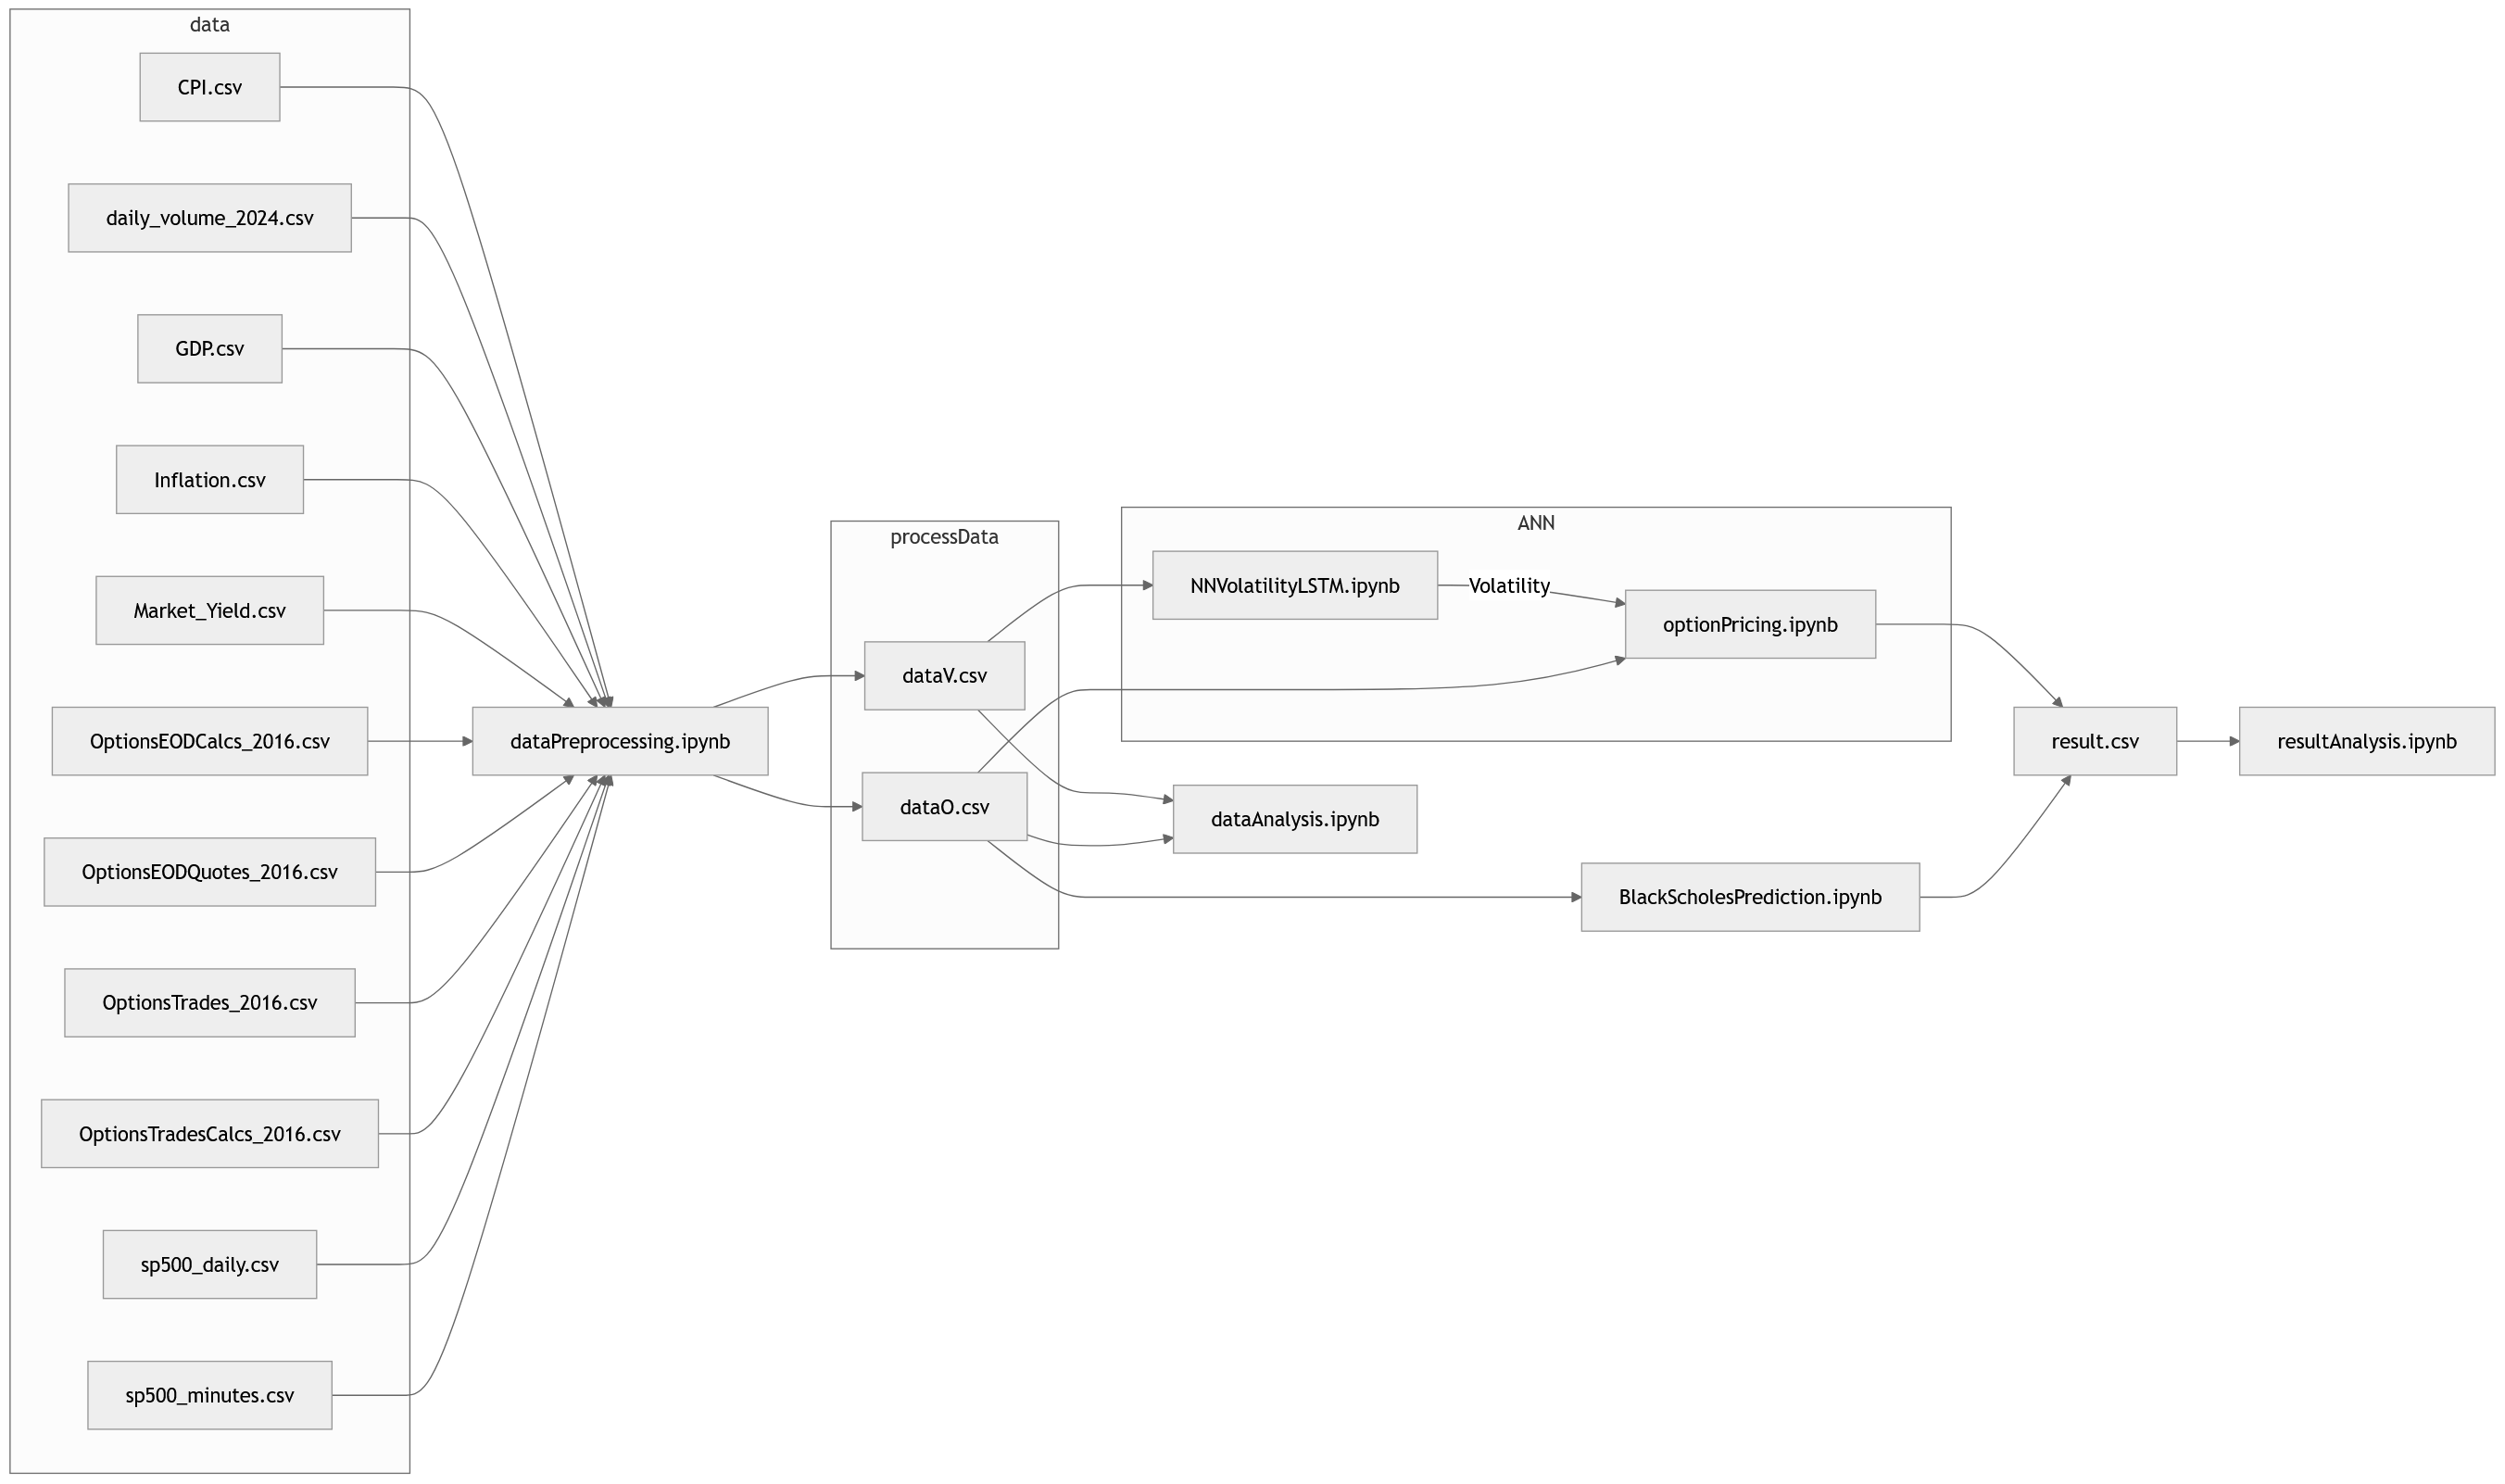
\includegraphics[width=0.9\textwidth]{img/structure.png}
            \end{center}

\newpage
\section*{Iteration 1}
\begin{flushright}
February 3, 2025
\end{flushright}
\hrule
\vspace{0.2in}

\subsection*{What Is New?}
\begin{itemize}
    \item Created and trained a ANN MLP model for option pricing, using Black-Scholes parameters to target option prices.
            
\begin{figure}[H]
  \centering
  \begin{minipage}[b]{0.45\textwidth}
    \centering
    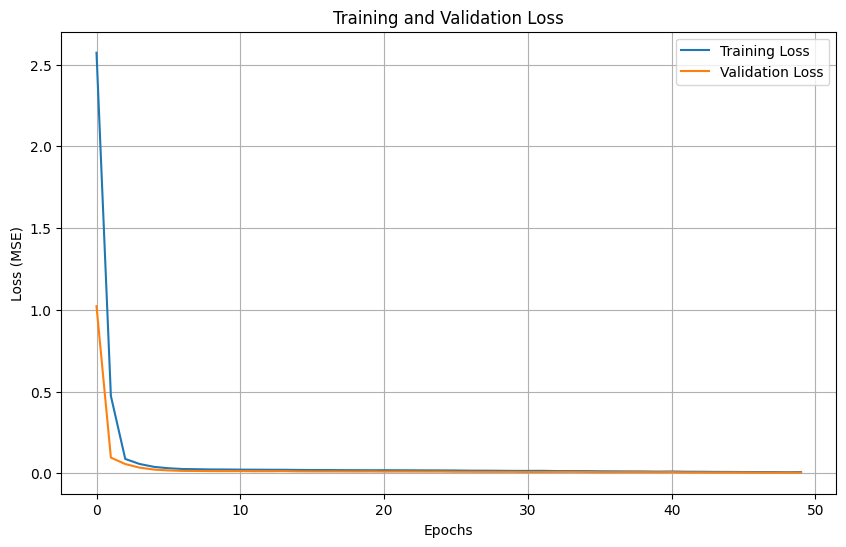
\includegraphics[width=\linewidth]{img/Loss_options_model.png} 
  \end{minipage}
  \hfill
  \begin{minipage}[b]{0.5\textwidth}
    \centering
    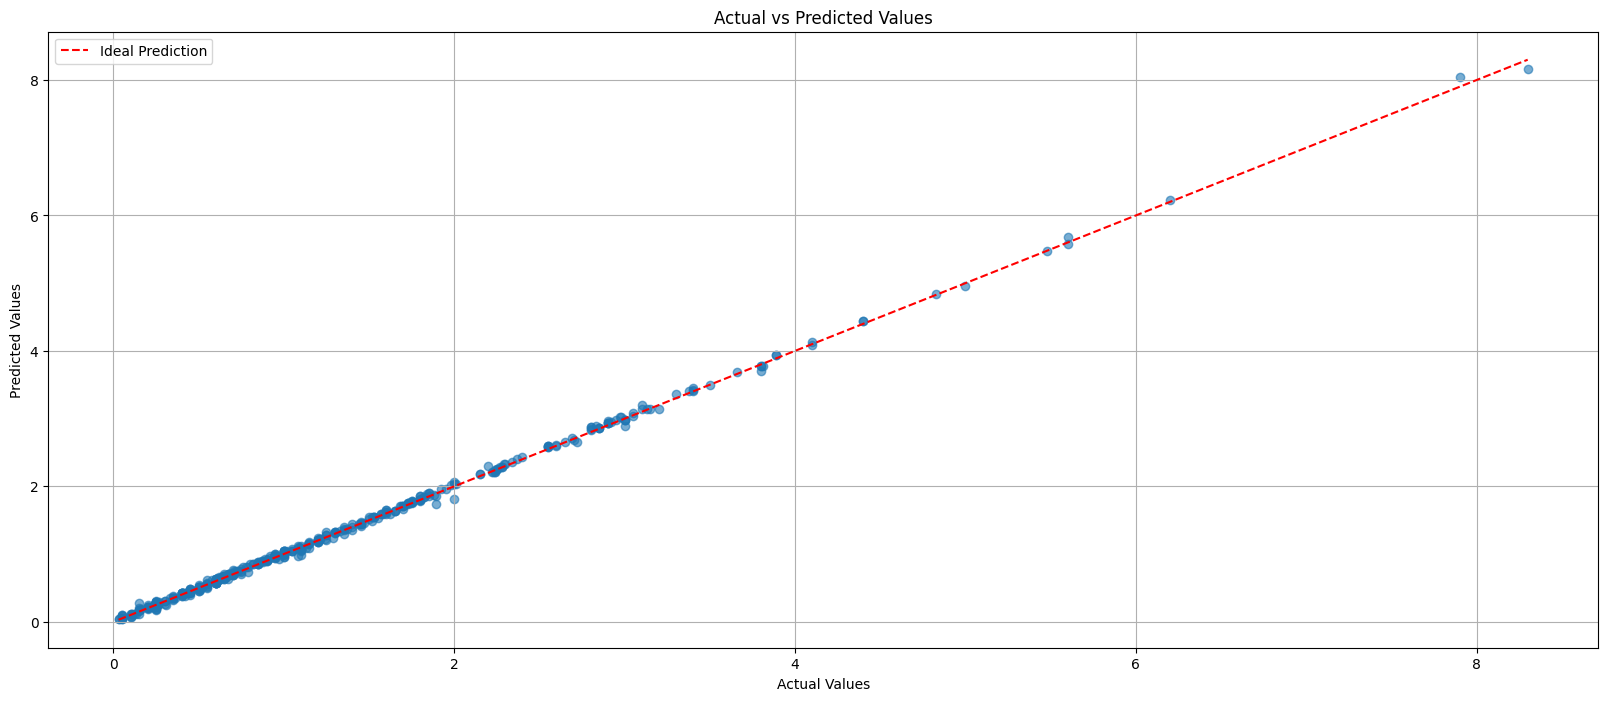
\includegraphics[width=\linewidth]{img/OPMreg.png}
  \end{minipage}
\end{figure}

    \item Compared the model's performance against Black-Scholes models:
            \begin{center}
            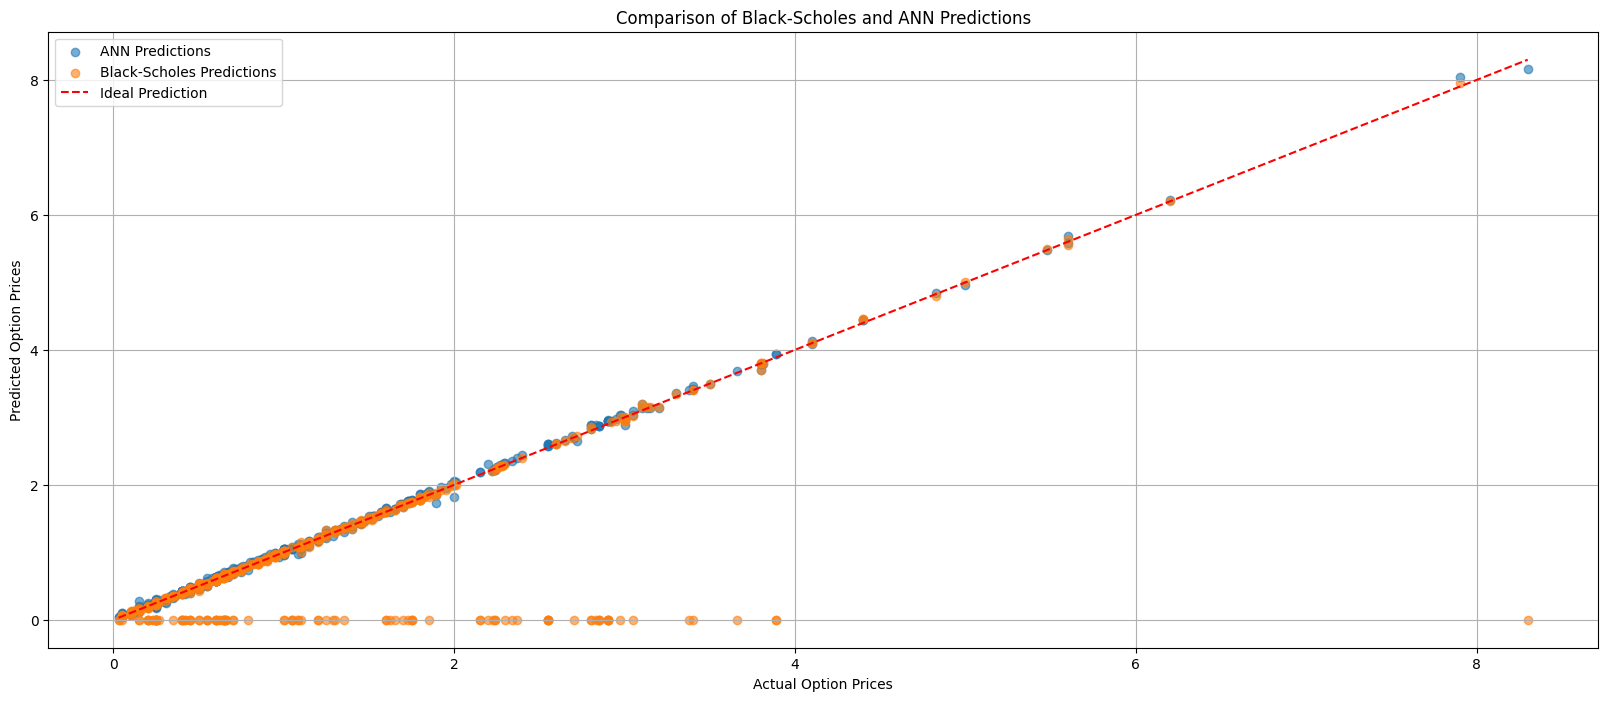
\includegraphics[width=0.8\textwidth]{img/BSvANN.png}
            \end{center}
            
    \item Started to build a custom LSTM model with NumPy. For now, I think Python allows better flexibility and development time than C++, while still maintaining decent performance using only NumPy. 
    I want the model to be compatible with TensorFlow formatting for easier use.
\end{itemize}

\subsection*{What Is Next?}
\begin{itemize}
    \item Finish the custom MLP model.
    \item Outliers suppression 
\end{itemize}

\newpage
\section*{Iteration 2}
\begin{flushright}
February 10, 2025
\end{flushright}
\hrule
\vspace{0.2in}
\subsection*{What Is New?}
\begin{itemize}
  \item First principle implementation of artificail neural network \textbf{multilayer perceptron}. Can be found here : /code\_/models/annModels.py
  \item \begin{verbatim}
  mlp = am.MLP(n_input=22, n_hidden1=64, n_hidden2=32, n_output=1)
  epochs = 5000
  learning_rate = 0.001
  
  #Training
  history = mlp.train(X_train_normalized, y_train, epochs, learning_rate)
  
  # Predict
  train_preds = mlp.forward(X_train_normalized)
  y_pred = mlp.forward(X_test_normalized)

  #---
  Final Training Loss: 0.41194406219492513
  Final Test Loss: 0.41460153925356924
  \end{verbatim}
  
  \begin{center}
    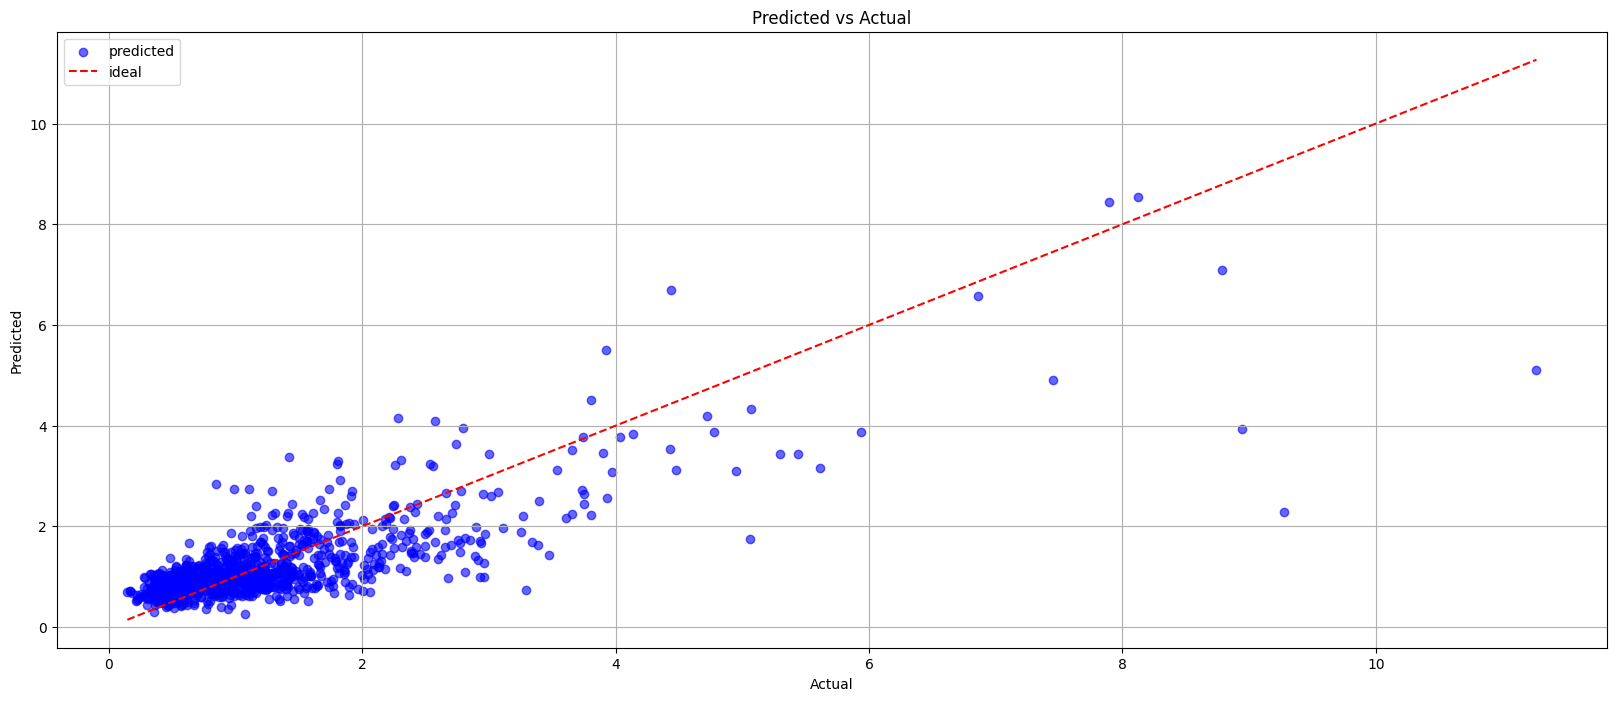
\includegraphics[width=0.8\textwidth]{img/custom_model_perf.png}
    \end{center}
\end{itemize}
\subsection*{What Is Next?}
\begin{itemize}
  \item Paramater optimization for custom model implementation ?
  \item Would a Transformer work better ? - \href{https://en.wikipedia.org/wiki/Transformer_(deep_learning_architecture)}{Wiki Transformer}
  \begin{itemize}
    \item Very likely, However, to get a working transformer model, the data volume is much more advanced than we currently use.
  \end{itemize}
\end{itemize}

\newpage
\section*{Iteration 3}
\begin{flushright}
February 17, 2025
\end{flushright}
\hrule
\vspace{0.2in}
\subsection*{What Is New?}
\begin{itemize}
  \item Finnish data gathering with scipt :/code\_/tools/getData.ipynb, all the assets data are gather in /data/stocks (around 200 symbols)
  \item Transformer implementation in progress
  \item Benchmark against LSTM model
  \item Paramater optimization for custom model implementation ?
\end{itemize}

\subsection*{What Is Next?}
\begin{itemize}
  \item Document on maths behind models (models.pdf)
\end{itemize}


\newpage
\section*{Iteration 4}
\begin{flushright}
February 24, 2025
\end{flushright}
\hrule
\vspace{0.2in}
\subsection*{What Is New?}
\begin{itemize}
  \item LSTM implementaiton in progress
  \item FFNN MLP and LSTM mathematics models
\end{itemize}

\subsection*{What Is Next?}
\begin{itemize} 
  \item Identifies specific aspect of volatility time series (mean reversion, volatility clustering, heavy tail)
  \item identifies drawback in LSTM architecture for specific financial time series
  \item Optimize model for financial time series 
  \item identify best loss function for volatility time series
\end{itemize}





\newpage
\section*{Iteration 5}
\begin{flushright}
March 3, 2025
\end{flushright}
\hrule
\vspace{0.2in}
\subsection*{What Is New?}
\begin{itemize}
  \item Data Work\begin{itemize}
    \item Compare to litterature
    \item Normalize data to improve models performances
    \item Select relevant feature to work with the model (clean confusion matrix)
  \end{itemize}
  \item Litterature about new/modify LSTM model for financial time series prediction
  \item Document on volatility model updated
\end{itemize}


\begin{center}
  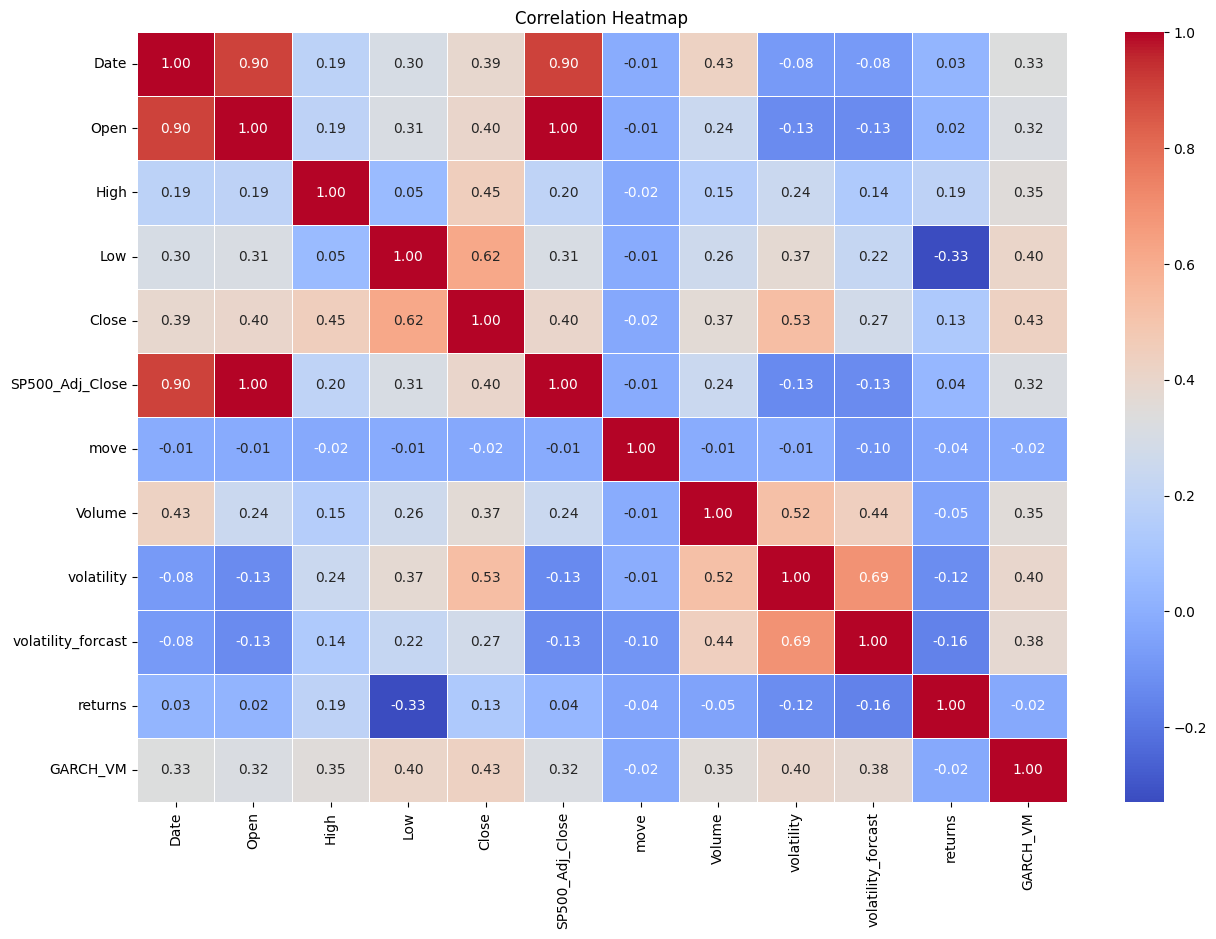
\includegraphics[width=0.7\textwidth]{img/corr_matrixS.png}
  \end{center}

\subsection*{What Is Next?}
\begin{itemize} 
  \item Improve mathematical relationship of LSTM models with litterature and financial time series properties.
  %\item 
 
\end{itemize}







\newpage
\section*{Iteration 6}
\begin{flushright}
March 10, 2025
\end{flushright}
\hrule
\vspace{0.2in}
\subsection*{What Is New?}
\begin{itemize}
  \item The volatility time series have some properties as for exemple \textbf{volatility clustering}. It implied that huge amplitude volatility periode are follow by small volatility changes and back to huge periode. The default LSTM network isn't aware of that so we can try to implement this in the forget gate to keep this informaiton inside the network.
  For instance we can propose a solution like this
  \[
  F_t = \sigma \left( W_f \cdot [H_{t-1}, X_t] + b_f \mathbf{- k \sigma_t} \right)
  \]

Where the new term $ k \sigma_t$ represente the a contante $k$ that is a leanring parameter to scale the impact on the network
and $\sigma_t$ that is the volatility estimation value.

\end{itemize}


\subsection*{What Is Next?}
\begin{itemize} 
  \item Implementaiton
  \item Benchmark against default LSTM and Black-Scholes
  \item Litterature
 
\end{itemize}




\newpage
\section*{Iteration 7}
\begin{flushright}
March 24, 2025
\end{flushright}
\hrule
\vspace{0.2in}

\subsection*{Litterature review}
\begin{enumerate}
  \item AT-LSTM: An Attention-based LSTM Model for Financial 
  Time Series Prediction\\
  \emph{Adding and attention layer to LSTM model. Appliyng weight to input feature thanks to an attention layer. Then, in a second stage, the attention model select all relevant features for LSTM input model.
  \begin{center}
    \begin{tabular}{c | c}
    \multicolumn{2}{c}{MAPE on DJIA} \\
    \hline
    LSTM & 0.00625 \\
    \hline
    AT-LSTM & 0.00486 \\
    %\hline
    \end{tabular}
  \end{center}
  }
  \item Improved Financial Predicting Method Based on Time Series Long Short-Term Memory Algorithm\\
  \emph{Automated capital prediction strategy, first by analysing the fluctuation and tail risk. Then by use ARIMA and Prophet models. Finally time series modeleing of the wavelet LSTM for a two part analysis of the linear separated wavelet and non-linear embedded wavelet to predict volatility. 
  }
  \begin{center}
    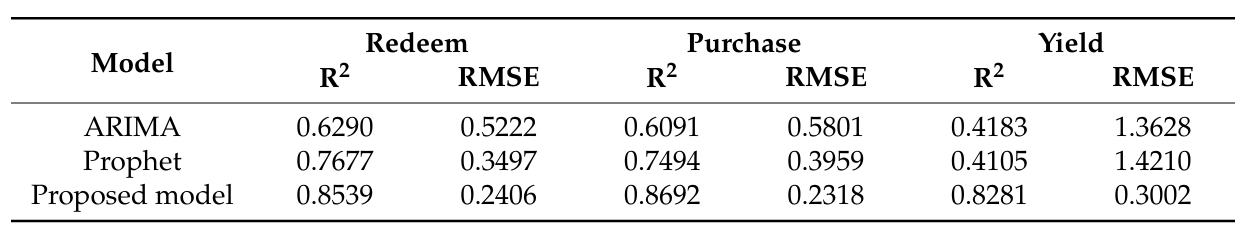
\includegraphics[width=0.7\textwidth]{img/res_lit_paper_1.png}
  \end{center}
 
  \item Prediction of Financial Time Series Based on LSTM Using Wavelet Transform and Singular Spectrum Analysis\\
  \emph{Imporove LSTM prediction capabilities by using data denoising methods including wavelet transformation (WT) and singular spectrum analysis (SSA) on the closing DJIA, divided in short, meduim and long term time periode.
  The LSTM data denoising performe better than raw data for data prediciton on all tree time periodes.
  }
  \begin{center}
    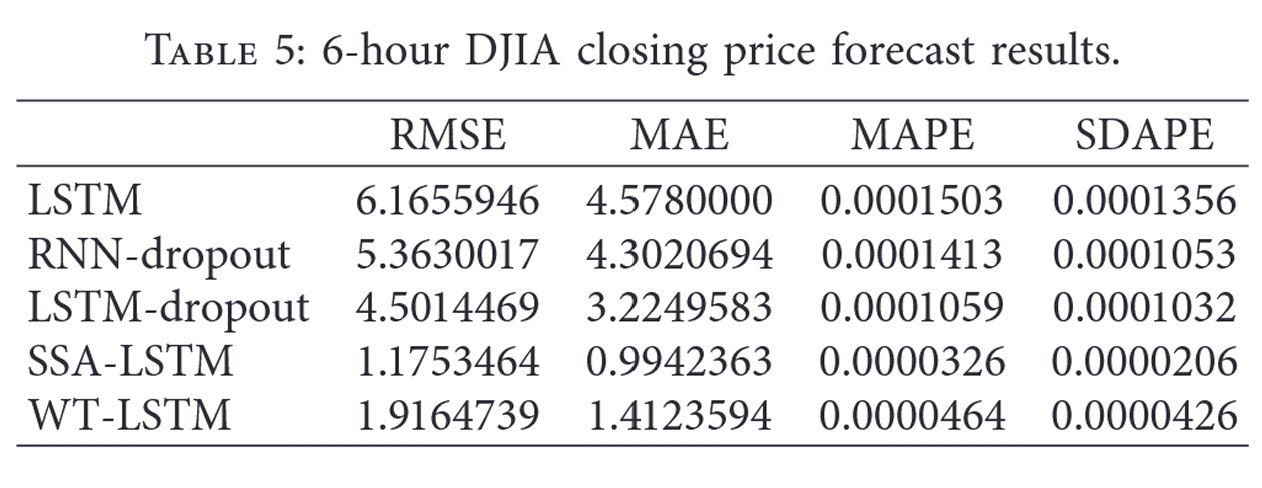
\includegraphics[width=0.7\textwidth]{img/res_lit_paper_2.png}
  \end{center}



  \item Black-Scholes-Artificial Neural Network : A novel option princing model\\
  \emph{Comparaison of multiple option pricing model and intruduction of a new model call BSANN, a basic ANN MLP model in [11-15-1] performing better than tranditionnal methodes.}

  \item Volatility forcasting using deep neural network with time-series feature embedding\\
  \emph{Propose a hybrid deep neural network model (HDNN). Encoding one-dimensionnal time-series data into two-dimensionnal GAF images to use a CNN with 2D concolutions layers, then performe feature embeding  and dense layers regression to predict the volatility}
  \begin{center}
    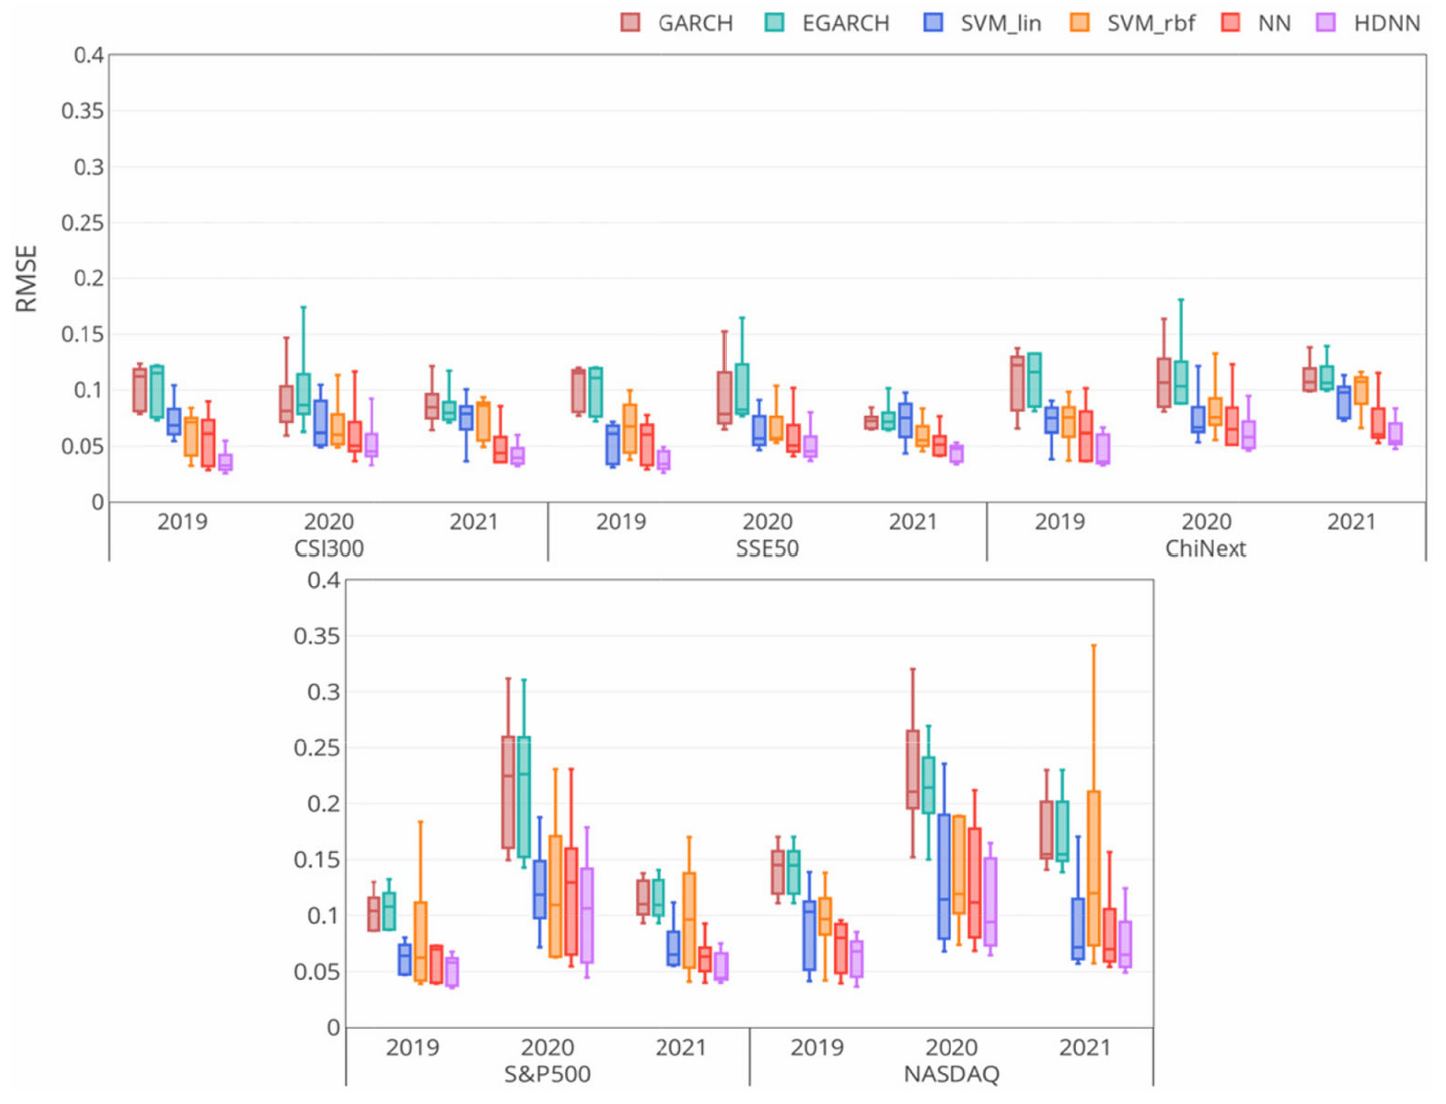
\includegraphics[width=0.6\textwidth]{img/res_lit_paper_3.png}
  \end{center}


  \item Volatility forcasting using deep recurrent neural networks as GARCH models\\
  \emph{Propose new method to predict volatility time series by using a combination of GARCH and and deep neural network. Also introduce a mehanisme to identifiy ideal sliding windows side for volatilty. With evaluation of GRU, LSTM, BiLSTM}
  \begin{center}
    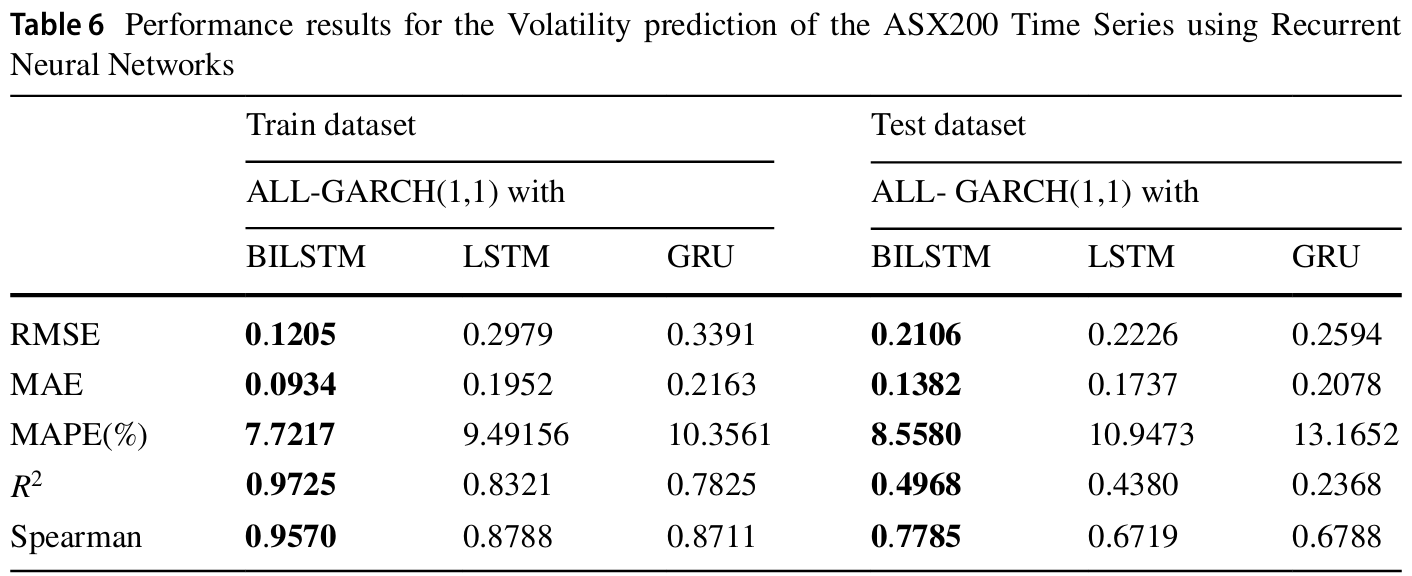
\includegraphics[width=0.7\textwidth]{img/res_lit_paper_4.png}
  \end{center}

  \item Machine Learning for Options Pricing: Predicting Volatility and Optimizing Strategies – Explore how ML models can outperform   traditional pricing models (like Black-Scholes), enhancing option traders' decision-making.\\
  \emph{}


  \item NEURAL NETWORK LEARNING OF BLACK-SCHOLES
  EQUATION FOR OPTION PRICING\\
  \emph{}

  \item Option Pricing with Deep Learning\\
  \emph{This paper propose a deep learning approach to option pricing with 3 models, 2 MLP(1\&2) and a LSTM model. MPL1 as a MLP predicting the option price, while MLP2 predicting the bid \& ask of the underlying price. Furthermore, LSTM model extimating volatility to feed its outpur to the MLP1 and then having a prediction of the option price.}
  \begin{center}
    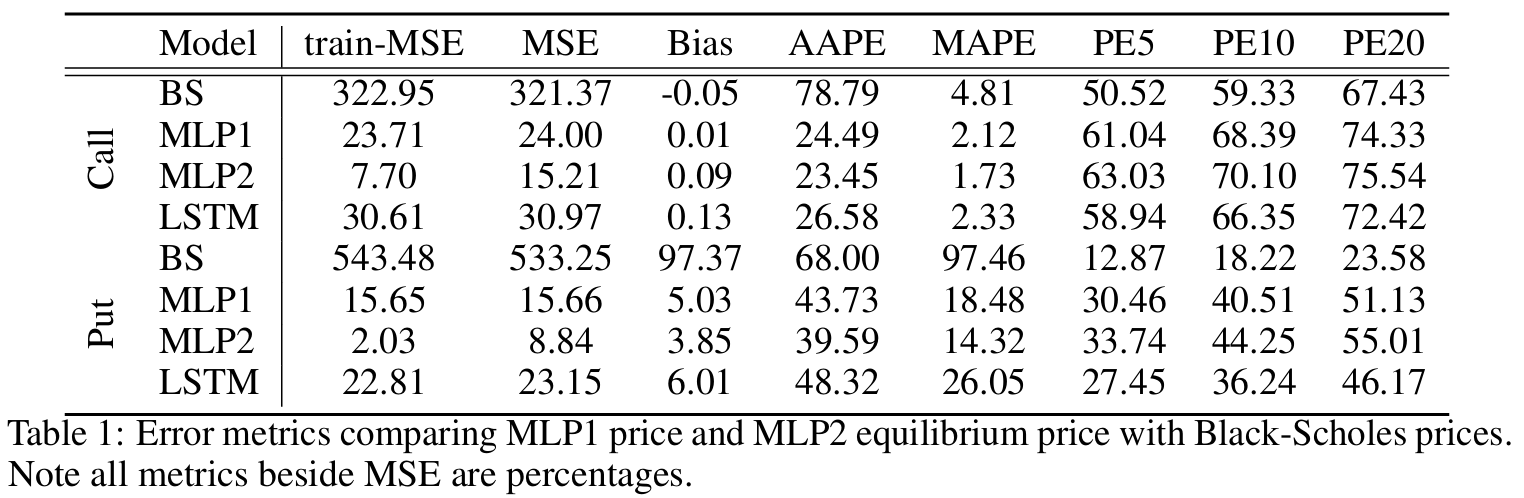
\includegraphics[width=0.7\textwidth]{img/res_lit_paper_5.png}
  \end{center}

  \item Volatility forecast using hybrid Neural Network models \\



\end{enumerate}




\newpage
\section*{Iteration 8}
\begin{flushright}
March 31, 2025
\end{flushright}
\hrule
\vspace{0.2in}

\subsection*{LSTM implementation}
Model architecture : [8-16-1]

\subsection*{Data work}
\begin{itemize}
  \item \textbf{Re-sizing of the data} - Data work\\
  In the file dataResize.csv the size of the data have been resize to 2 weeks per exemple.
    \begin{center}
    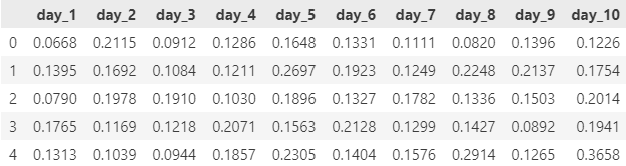
\includegraphics[width=0.7\textwidth]{img/dataR.png}
    \end{center}

  \item \textbf{Data seasonality} - Analysis\\
  Analysis reccurent pattern in dataResize to use the 10-days seasonnality.
  \begin{figure}[H]
    \centering
    \begin{minipage}[b]{0.49\textwidth}
      \centering
      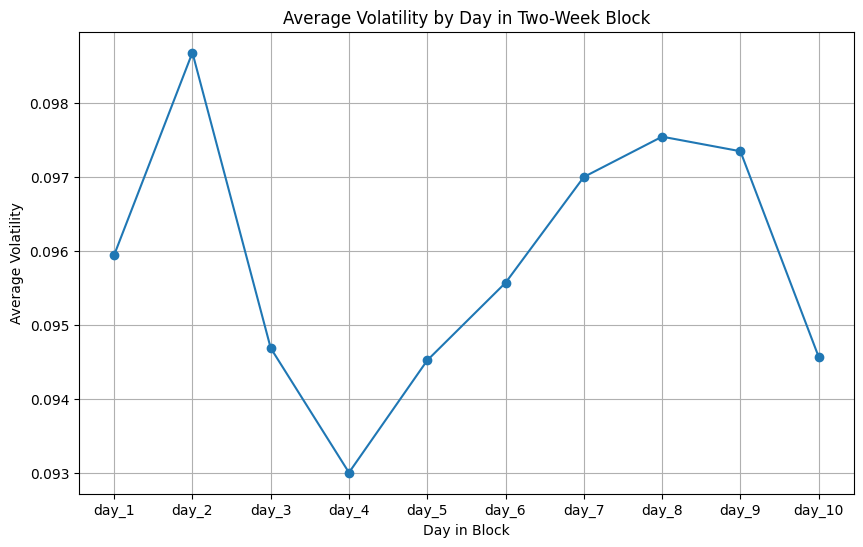
\includegraphics[width=\linewidth]{img/10avg_vol.png} 
    \end{minipage}
    \hfill
    \begin{minipage}[b]{0.50\textwidth}
      \centering
      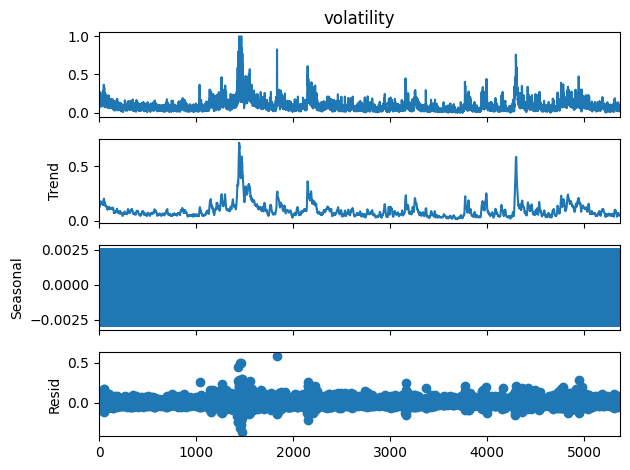
\includegraphics[width=\linewidth]{img/seaso.png}
    \end{minipage}
  \end{figure}



  \item \textbf{De-noising (Wavelet)} - Data work\\
  De-noising the raw data to better capture the trend in the time serie
  \begin{center}
    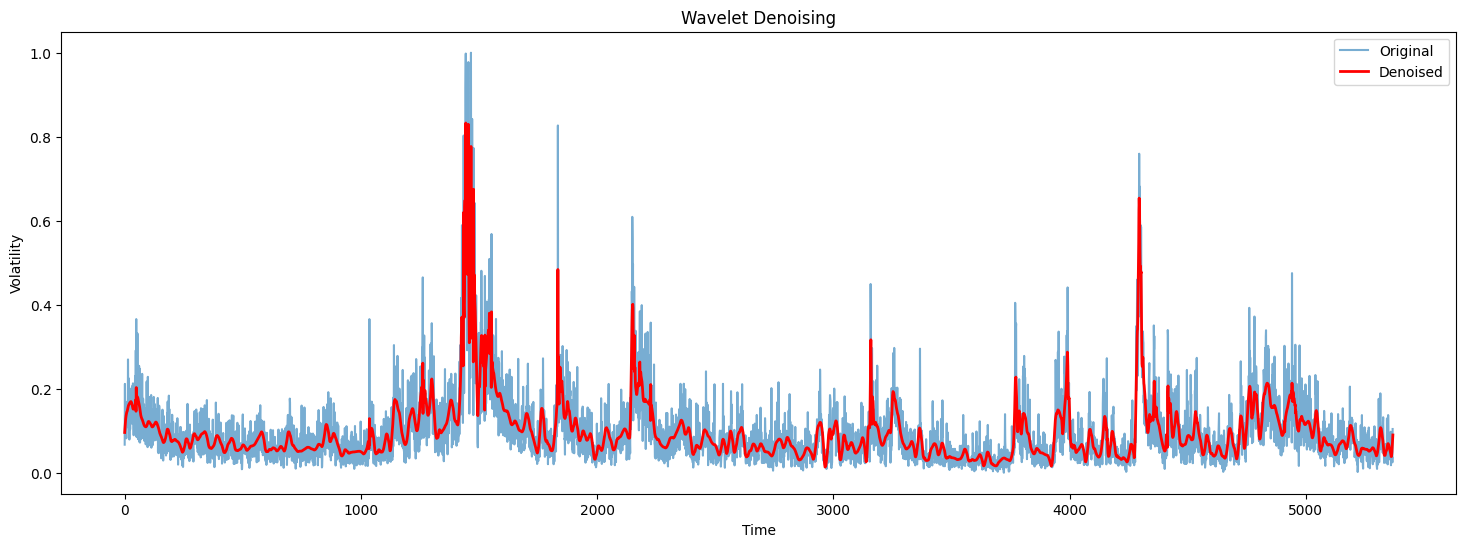
\includegraphics[width=0.8\textwidth]{img/wavelet.png}
    \end{center}
  \item \textbf{Sliding windows} - Analysis\\
  Papers : \href{https://link.springer.com/content/pdf/10.1007/s00180-023-01349-1.pdf}{Volatility forcasting using deep recurrent neural networks as GARCH models}\\
  and \href{https://www.sciencedirect.com/science/article/pii/S1053811920305978}{Single-scale time-dependent window-sizes in sliding-window dynamic funcitonal connectivity analysis}
  
\end{itemize}


\subsection*{Statistical models}
\begin{itemize}
  \item ARIMA
  \item GRU
  \item BiLSTM
\end{itemize}







\newpage
\section*{Iteration 9}
\begin{flushright}
April 7, 2025
\end{flushright}
\hrule
\vspace{0.2in}

%\subsection*{LSTM model}
\subsection*{Sliding window}
\subsubsection*{Implementation}
Implementation of static sliding windows on the volatility time serie 
  \begin{center}
  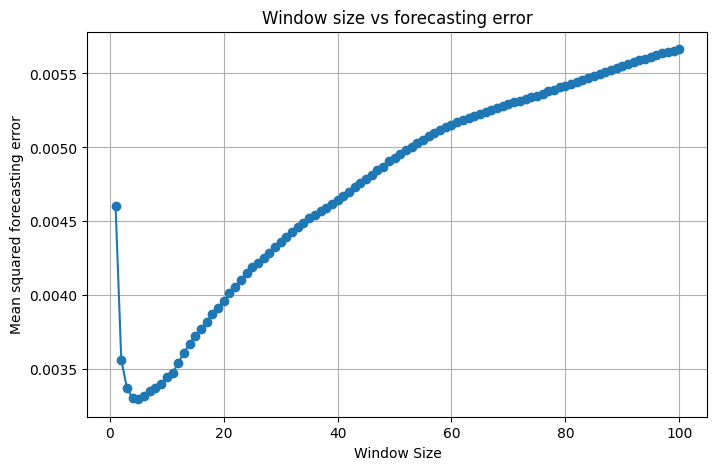
\includegraphics[width=0.8\textwidth]{img/win_err.png}
  \end{center} %changer la vol en close/returns
  Best window size given by the EMD is currently 5 days (a trading week) with MSE estimator.


\subsubsection*{Improvement - Dynamic sliding window}




\newpage
\section*{Iteration 10}
\begin{flushright}
April 14, 2025
\end{flushright}
\hrule
\vspace{0.2in}

\subsection*{LSTM}

Need to improve LSTM performance, not as good as TensorFlow implementation.

\subsection*{Sliding Window}
The dynamic sliding vector may cause a problem with the LSTM vectore size.




\end{document}
